\section{The solution}
\label{sec:middleware_architecture}

% Description of the overall architecture designs
% Argue for tactics used to archieve the QASes
% Discuss the trade-offs
This section outlines the proposed technological solution for the medium-sized cattle farm. The design integrates various hardware and software components such as sensors, Java-based subsystems, message bus for middleware communication and Big data server for storing data. The whole purpose of this solution is to address the unique needs of the farm's operations which include animal care, feed management, and sales.

\subsection{\textbf{System Overview}}
The proposed system integrates biometric and feed monitoring, automated feeding, and resource management, ensuring efficiency and sustainability in farm operations. It is designed to manage around 100 animals, utilizing 200 to 300 sensors for various monitoring purposes such as monitoring the heart rate of cows, temperature or humidity of silos. In order for the system to be successful, continuous interoperability among various departments and their Java-based subsystems need to exist. Therefore, a robust middleware communication system facilitated by a central message bus was chosen to be used as the optimal architecture. \newline
\begin{figure*}[!ht]
    \centering
    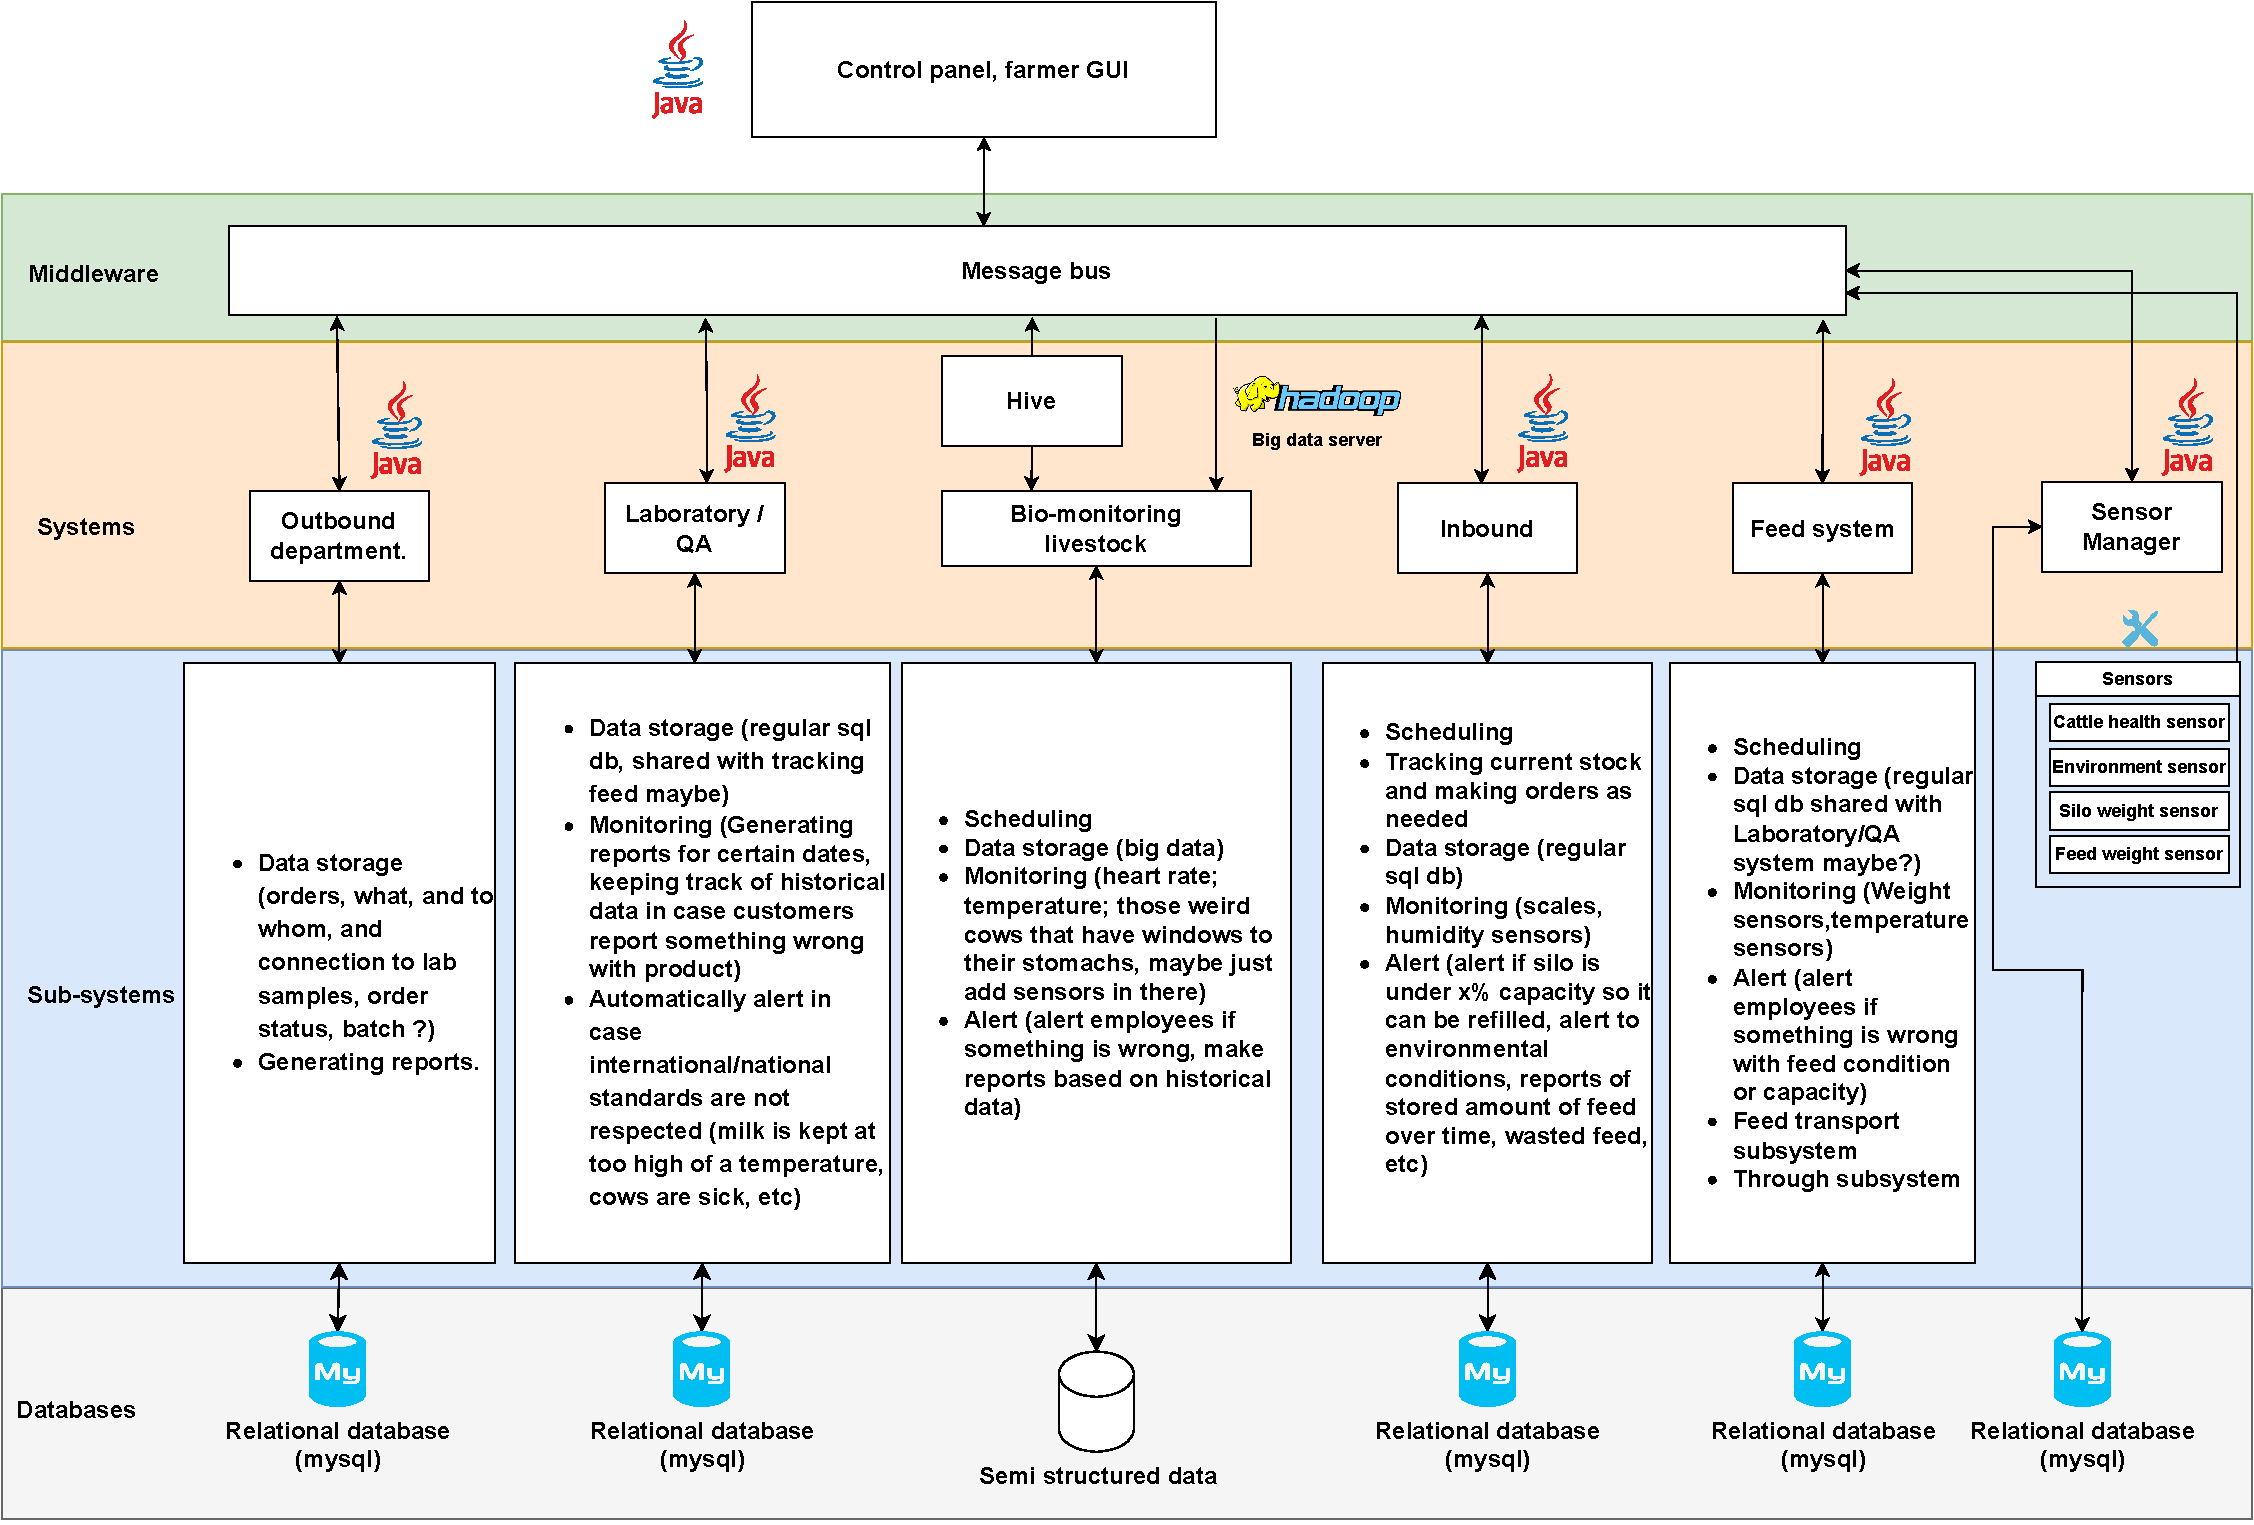
\includegraphics[width=\textwidth]{Images/architecture.pdf}
    \caption{The proposed architecture}
    \label{fig:systemArch}
\end{figure*}

Figure \ref{fig:systemArch} depicts the initial architecture that was drafted for the system. A few of these systems are not present in the final system implementation, but there will be enough implementation to show how the system adheres to the required quality attributes which are specified in the quality attribute scenarios from section \ref{sec:qas} and how the rest of the system can be implemented.
\subsection{\textbf{Middleware and Communication}}
For an Industry 4.0 system the middleware is the center of attention. From related work knowledge was obtained that highlighted the need for interoperability between different systems, this is where the message bus comes into play. \vspace{2mm} \\
Apache Kafka \cite{Apache2022Connect} has been selected for real-time data handling and as a central component of the message bus due to its distinct advantages in large-scale applications. Kafka offers high throughput and low latency, making it ideal for managing huge streams of sensor data in real-time. Furthermore, Kafka's ecosystem, including Kafka Connect, enables the efficient processing of big data, an essential requirement for the project. \vspace{2mm} \\

The distributed nature of Kafka uses multiple brokers, which for Kafka means that it has several servers to recieve and send data. This helps avoid a single point of failure and ensures system reliability. Kafka uses multiple tactics to achieve it's fault tolerance, one being replication of data across multiple brokers, which ensures if a broker is lost no data will be lost \cite{AltexSoft_2022}. This behavior is needed for the QAS described for availability in the system.
Besides affecting the QAS, Kafka also has great support for a variety of different systems and languages \cite{AltexSoft_2022}, which will support the interoperability of the system. \vspace{2mm}

The main downsides of using Kafka is the technological complexity and lack of management and monitoring tools. This presents a challenge and necessitates additional effort in system administration. Despite these challenges, Kafka's performance, scalability, and the ability to integrate with various technologies such as Hadoop for big data needs, make it the most suitable choice for the system. \vspace{2mm}


\subsection{\textbf{Subsystem Integration}}
Each department's Java-based subsystem operates through the middleware message bus, carrying out specific functions that are essential for each department needs. \vspace{2mm}\\
The choice of using Java-based subsystems can be described by several factors. Firstly, Java is an object-oriented programming language which makes for easier implementation as it allows for breaking the code into smaller, more manageable parts. \cite{Team_2022}.
Another important feature of Java is the ability to run on many devices, with different operating systems and hardware configurations. The interoperability of Java is what allows us to develop with a wide variety of systems. It supports \textit{deployability} by being platform independent and having standardized packaging. \vspace{2mm} \\
Java also provides automatic garbage collection, which helps it manage memory efficiently \cite{Team_2022}. This supports the \textit{availability} of the system by reducing the likelihood of memory errors.
Even though Java supports some of the system requirements, it also has tradeoffs. Just as automatic garbage collection is a plus, it also affects performance by always running in the background, where in languages like C or C++ this does not happen \cite{Team_2022}. \vspace{1mm}

\subsection{\textbf{Sensor Implementation}}
The farm’s operations are monitored by an array of sensors that perform various functions. Cattle health sensors monitor vital signs such as heart rate and body temperature, providing critical data for early illness detection. Environmental sensors monitor conditions on the farm, including temperature and humidity levels within the fields, the barns and silos. Silo weight sensors monitor and measures the amount of feed stored, and feed weight sensors keep track of distribution of feed to the cattle farm. \vspace{2mm} \\
All sensors are connected to a central middleware message bus, which uses Kafka to stream sensor data. This design allows the data to be analyzed and ingested into Hadoop Distributed file system (abriviated HDFS for later reference), from where it can be queried and used in reports. Kafka’s distributed nature and streaming capabilities enable the system to handle the influx of data from potentially hundreds of sensors without loss of information or delay, ensuring that the most current data is always available for decision-making processes. \vspace{2mm}

\subsection{\textbf{Database Management}}
A relational database using MySQL is employed across the Java-based subsystems, providing a consistent framework for data management.
The use of MySQL which is a relational database makes sense for the most of the subsystems in the architecture, because here it is not necessary to store live data but more historical data. MySQL also supports some of the quality attributes for the system. Just like Java, MySQL is platform independent \cite{Blue}, which means it supports \textit{deployability} by requiring no modification regardless of where it is running.
The main disadvantage of MySQL is the poor performance when exposed to high loads \cite{Blue}. Looking at the specified architecture there is  another system for storing the sensor data, which will handle the larger amounts of data better.

\subsection{\textbf{Bio-monitoring Livestock System}}
\subsubsection{Hardware}
Sensors are attached to each animal for monitoring temperature and heart rate, ensuring 24/7 health surveillance.\vspace{2mm}
\subsubsection{Software}
A Big Data architecture is employed, leveraging Kafka for robust data ingestion into HDFS. Kafka serves as a high-throughput distributed messaging system, capable of handling the streams of sensor data in real-time. It is chosen for its fault tolerance, durability, and ability to process data streams as continuous flows, which is critical for timely and accurate monitoring of livestock health.\vspace{2mm}
\subsubsection{Functionality}
The system operates continuously, utilizing Machine Learning to analyze the data and detect early signs of illness, notifying in time the animal care department. Kafka's immediate and efficient processing of data ensures speed and time efficiency to the system.\vspace{2mm}


\subsection{\textbf{Feed System}}
\subsubsection{Hardware}
Automated feeders equipped with sensors to control and monitor feed distribution.\vspace{2mm}
\subsubsection{Software}
Java-based control system to manage feeding operations, ensuring consistent and accurate feeding.\vspace{2mm}
\subsubsection{Functionality}
Real-time 24/7 monitoring with error detection and alerting mechanisms for immediate handling of issues.

\subsection{\textbf{Inbound System}}
\subsubsection{Hardware}
Feed silos equipped with scales and humidity sensors.\vspace{2mm}
\subsubsection{Software}
Java and MySQL manage data capturing and processing, facilitating efficient feed utilization and ordering.\vspace{2mm}
\subsubsection{Functionality}
Regular monitoring and data capture optimize feed management and resource planning.

\subsection{\textbf{Outbound System}}
Developed in Java, this MVC application manages customer orders, linking them with laboratory samples for efficient tracking and processing.

\subsection{\textbf{Hardware and Software Synergy}}
The sensor data is being mimicked by a Java application, that can simulate live sensor data. This allows for the posibility of evaluating on the systems capabilities in regards to data throughput.

\subsection{\textbf{Integration with HFDS}}
The integration of Kafka with the HDFS is a necessary decision to manage the large volumes of data generated by the biometric and environmental sensors. HDFS provides a reliable and scalable storage solution, capable of handling vast amounts of data while ensuring data integrity and accessibility. This integration allows for efficient data processing, storage, and retrieval, which are crucial for the real-time monitoring and analysis required in the bio-monitoring livestock system. \vspace{2mm} \\
HDFS supports several of the quality attributes required by the system. The main reasoning behind the use of it is because of the limited storage possibilites by MySQL, in HDFS it is possible to store extremely large amounts of data.
HDFS enhances the \textit{availability} by implementation of fault tolerance. As Kafka can replicate the data, same goes for HDFS, which means that it replicates the data across several nodes (physical computers) in a cluster (a group of physical computers) \cite{AltexSoft_2022a}. When a node fails no data is therefore lost, this refers to the tactic \textit{voting} which defines replication as a way of detecting faults \cite{Bass2012Software}.
HDFS is also able to scale horizontally which allows for a simple way to add more capacity for storing data. HDFS is located within the Apache ecosystem which provides a handful of different technologies for different use cases \cite{AltexSoft_2022a}, this improves the interoperability of the system as HDFS is able to communicate with various different technologies. As for the deployability of HDFS it is built on Java, which as mentioned can run on any system or hardware.\vspace{2mm} \\
When using HDFS it is important to consider that the files that are being stored are not too small. This is a disadvantages of HDFS, it has very poor handling of small files, in which case it is better to use SQL.
HDFS also has its own processing when trying to read data called MapReduce, which can be very slow and resource intensive when trying to process big data. Using Apache Hive can help aleviate this issue. Apache Hive is a data warehousing solution built on top of Apache Hadoop. It is designed to manage and query large datasets residing in distributed storage using a SQL-like syntax. Hive is particularly useful in systems that involve processing and analyzing big data, such as the sensor data in our project \cite{ApacheHive}.
The one downside that is provided by Hive is it doesnt handle real-time data querying, so in this system Hive would be used for looking at historical data \cite{ApacheHive}. Therefore the need for live data from the sensors is obtained from an intermediate data storage in the message bus (Kafka).

\subsection{\textbf{Containerization using Docker}}
For running the system it was containerized using Docker. Docker is a piece software that allows an open platform for developing, shipping and running applications \cite{Docker2022What}. It packages up code and its dependencies, which ensures that the applications run quickly and reliably from one environment to another \cite{Docker2022What}.
For the architecture proposed in the solution, each system has its own container and with all the systems containerized, it is possible to perform tests on the system using a single machine.\vspace{2mm} \\ Containerization helps isolate each system and therefore reducing conflicts between systems. Docker makes use of a few tactics to adhere to these principles that are connected to the \textit{deployability} QA. For managing the deployment pipeline it makes use of the \textit{Script deployment command} tactic which describes a script can do all the steps necessary for executing the deployment of the system as a whole \cite{Bass2012Software}. For managing the deployed system it also makes use of the \textit{Pacakge dependencies} which essentially describes how it packages the system, that leads to containerization \cite{Bass2012Software}.


\subsection{\textbf{Discussion on Trade-offs}}
The selection of Kafka and HDFS, while beneficial for handling big data and ensuring scalability, faces trade-offs. The complexity of Kafka gives rise to the need of complicated technological knowledge and more detailed system management. Additionally, the start setup and maintenance of the Hadoop ecosystem require crucial resources and expertise. These trade-offs and challenges are justified by the long-term benefitial existence of a scalable and flexible system capable of adapting to the evolving farming needs.
As for the use of Docker, some of the tradeoffs from Kafka and HDFS are also relevant here. This includes the inital added complexity for setting it up and in general expertise within the domain is needed for setup \cite{Gover_2023}. The tradeoffs are justified by the positives Docker provides which outweighs the negatives.